\documentclass[11pt,answers]{exam}

% Load useful packages
% Read in necessary packages
\usepackage{import}
\usepackage{amsmath}
\usepackage{amsfonts}
\usepackage{amssymb}
\usepackage{graphicx}
\usepackage{hyperref}
\usepackage{color}

% Set various options for exam package
\shadedsolutions % defines the style of the solution environment

% Set lesson name, etc.
\newcommand{\coursename}{Math 312}
\newcommand{\lessonname}{Problem Set 1}
\newcommand{\duedate}{28 January}
\newcommand{\names}{Tate Maki-Waller, Sam Gleason, Ian Gallmeister}

% Set headers/footers to look nice
\pagestyle{headandfoot}
\firstpageheader{\textbf{\large \coursename\ \lessonname}}{}{\textbf{\large Due \duedate}}
\firstpageheadrule
\runningheader{\textbf{\large \coursename\ \lessonname}}{}{\textbf{\large Due \duedate}}
\runningheadrule
\firstpagefooter{\names}{}{Page \thepage\ of \numpages}
\firstpagefootrule
\runningfooter{\names}{}{Page \thepage\ of \numpages}
\runningfootrule

% Define commands related to marking up content
\newcommand{\source}[1]{}

% Define commands related to general mathematical style
\renewcommand{\exp}[1]{e^{#1}}

%%%%%%%%%%%%%%%%%%%%%%%%%%%%%%%%%%%%%%%%%%%%%%%%%%%%%%%%%%%%

\begin{document}
\begin{questions}

\question Solve the initial value problem $dP/dt = e^{-t}\sin(4t), \: P(0) = 2$. Plot the solution for a long enough time to discern the long-term behavior. Discuss the long-term behavior by analyzing the formula for the solution and providing a graph.

\begin{solution}
Looking at the differential equation, it is apparent that it needs to be solved using integration by parts.  After using IBP, there is another integral created that also needs to be solved with integration by parts.  The integral resulting from the second use of IBP is the original integral with a coefficient, and we can subtract that over to the other side to get all integrals on one side.  Then we divide out the coefficient and apply the initial condition to find a value for $C$.
\begin{align*}
\frac{dP}{dt} &= e^{-t}\sin{(4t)}, \: P(0) = 2 \\
\int e^{-t}\sin{(4t)} dt &= \\
&u = \sin{4t} \hbox{\hspace{4.5em}} v = -e^{-t} \\ %futz with formatting!
&du = 4\cos{(4t)}dt \hbox{\hspace{2em}} dv = e^{-t} dt \\
\int e^{t}\sin{(4t)} dt &= -e^{-t}\sin{4t)} + 4\int e^{-t}\cos{(4t)}\\
&u = \cos{4t} \hbox{\hspace{5.5em}} v = -e^{-t} \\ %futz with formatting!
&du = -4\sin{(4t)}dt \hbox{\hspace{2em}} dv = e^{-t} dt \\
\int e^{-t}\sin{(4t)} dt &= -e^{-t}\sin{(4t)} - 4 e^{-t}\cos{(4t)} - 16\int e^{-t}\sin{(4t)} \\
17 \int e^{-t}\sin{(4t)} dt &= -e^{-t}\sin{(4t)} - 4 e^{-t}\cos{(4t)} \\
\int e^{-t}\sin{(4t)} dt &= \frac{-1}{17}\left(-e^{-t}\sin{(4t)} + 4 e^{-t}\cos{(4t)}\right) + C \\
\\
P(0) = 2 &= \frac{-1}{17}\left(-e^0\sin{0} + 4e^{0}\cos{0}\right) + C \\
2 &= C - \frac{4}{17} \\
C &= 2 + \frac{4}{17} = \frac{38}{17}
\\
\int e^{-t}\sin{(4t)} dt &= \frac{-1}{17}\left(-e^{-t}\sin{(4t)} + 4 e^{-t}\cos{(4t)}\right) + \frac{38}{17}
\end{align*}
\centerline{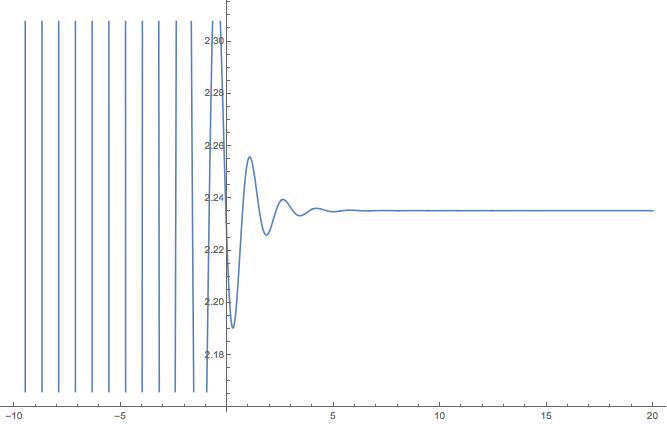
\includegraphics[width = 3in]{ps1p4.png}}

Because $e^t$ goes to infinity, $e^{-t}$ goes to 0 and the function value goes to $C$, or $38/17$.

\end{solution}



\end{questions}
\end{document}